\documentclass[11pt]{article}
\usepackage{latexsym}
\usepackage{amsmath}
\usepackage{amssymb}
\usepackage{amsthm}
\usepackage{epsfig}
\usepackage{bm}
\usepackage{scrextend}
\usepackage[tight]{subfigure}

\usepackage{amsmath}
% \usepackage{algorithmicx}
\usepackage{algorithm}
\usepackage{algpseudocode}

\DeclareMathOperator*{\minimize}{min}
\DeclareMathOperator*{\maximize}{max}
\DeclareMathOperator{\sign}{sign}


 %on linux you may need to run sudo apt-get install texlive-full to install algorithm.sys

\usepackage{verbatim}

\newcommand{\handout}[5]{
  \noindent
  \begin{center}
  \framebox{
    \vbox{
      \hbox to 5.78in { {#1} \hfill #2 }
      \vspace{4mm}
      \hbox to 5.78in { {\Large \hfill #5  \hfill} }
      \vspace{2mm}
      \hbox to 5.78in { {\em #3 \hfill #4} }
    }
  }
  \end{center}
  \vspace*{4mm}
}

\newcommand{\lecture}[5]{\handout{#1}{#2}{#3}{#4}{#5}}
\newcommand{\collision}[0]{\mathrm{collision}}
\newcommand{\nocollision}[0]{\overline{\collision}}
\newcommand{\argmax}[1]{\underset{#1}{\operatorname{arg}\,\operatorname{max}}\;}
\newcommand{\argmin}[1]{\underset{#1}{\operatorname{arg}\,\operatorname{min}}\;}

\newcommand*{\QED}{\hfill\ensuremath{\square}}

\newtheorem{theorem}{Theorem}
\newtheorem{corollary}[theorem]{Corollary}
\newtheorem{lemma}[theorem]{Lemma}
\newtheorem{observation}[theorem]{Observation}
\newtheorem{proposition}[theorem]{Proposition}
\newtheorem{definition}[theorem]{Definition}
\newtheorem{claim}[theorem]{Claim}
\newtheorem{fact}[theorem]{Fact}
\newtheorem{assumption}[theorem]{Assumption}
\newtheorem{note}[theorem]{Note}


% 1-inch margins, from fullpage.sty by H.Partl, Version 2, Dec. 15, 1988.
\topmargin 0pt
\advance \topmargin by -\headheight
\advance \topmargin by -\headsep
\textheight 8.9in
\oddsidemargin 0pt
\evensidemargin \oddsidemargin
\marginparwidth 0.5in
\textwidth 6.5in

\parindent 0in
\parskip 1.5ex
%\renewcommand{\baselinestretch}{1.25}

\begin{document}

\lecture{Statistical Techniques in Robotics (16-831, S21)}{Lecture \#07
  (Wednesday, February 24)}{Lecturer: Kris Kitani}{Scribes: Haowen Shi, Fan Jia}{Online Convex Optimization (FTRL, OMD)}

\section{Review}
%This section serves as a review of the previous lecture and any other context required to frame the content of the current lecture. 

%You may format the scribes in any way you like, aside from changing font style, size and page format. Please use subsections and paragraphs to increase the readability of your notes.

%Length requirement 1-2 pages.
In the last lecture, we studied a generalized framework of online learning algorithms called \textit{Online Convex Optimization} (OCO) \cite{shalev2011online}, as shown in Fig. \ref{fig:oco_1}. \\

\begin{figure}[h]
\centering
\begin{minipage}{.6\textwidth}
    \centering
    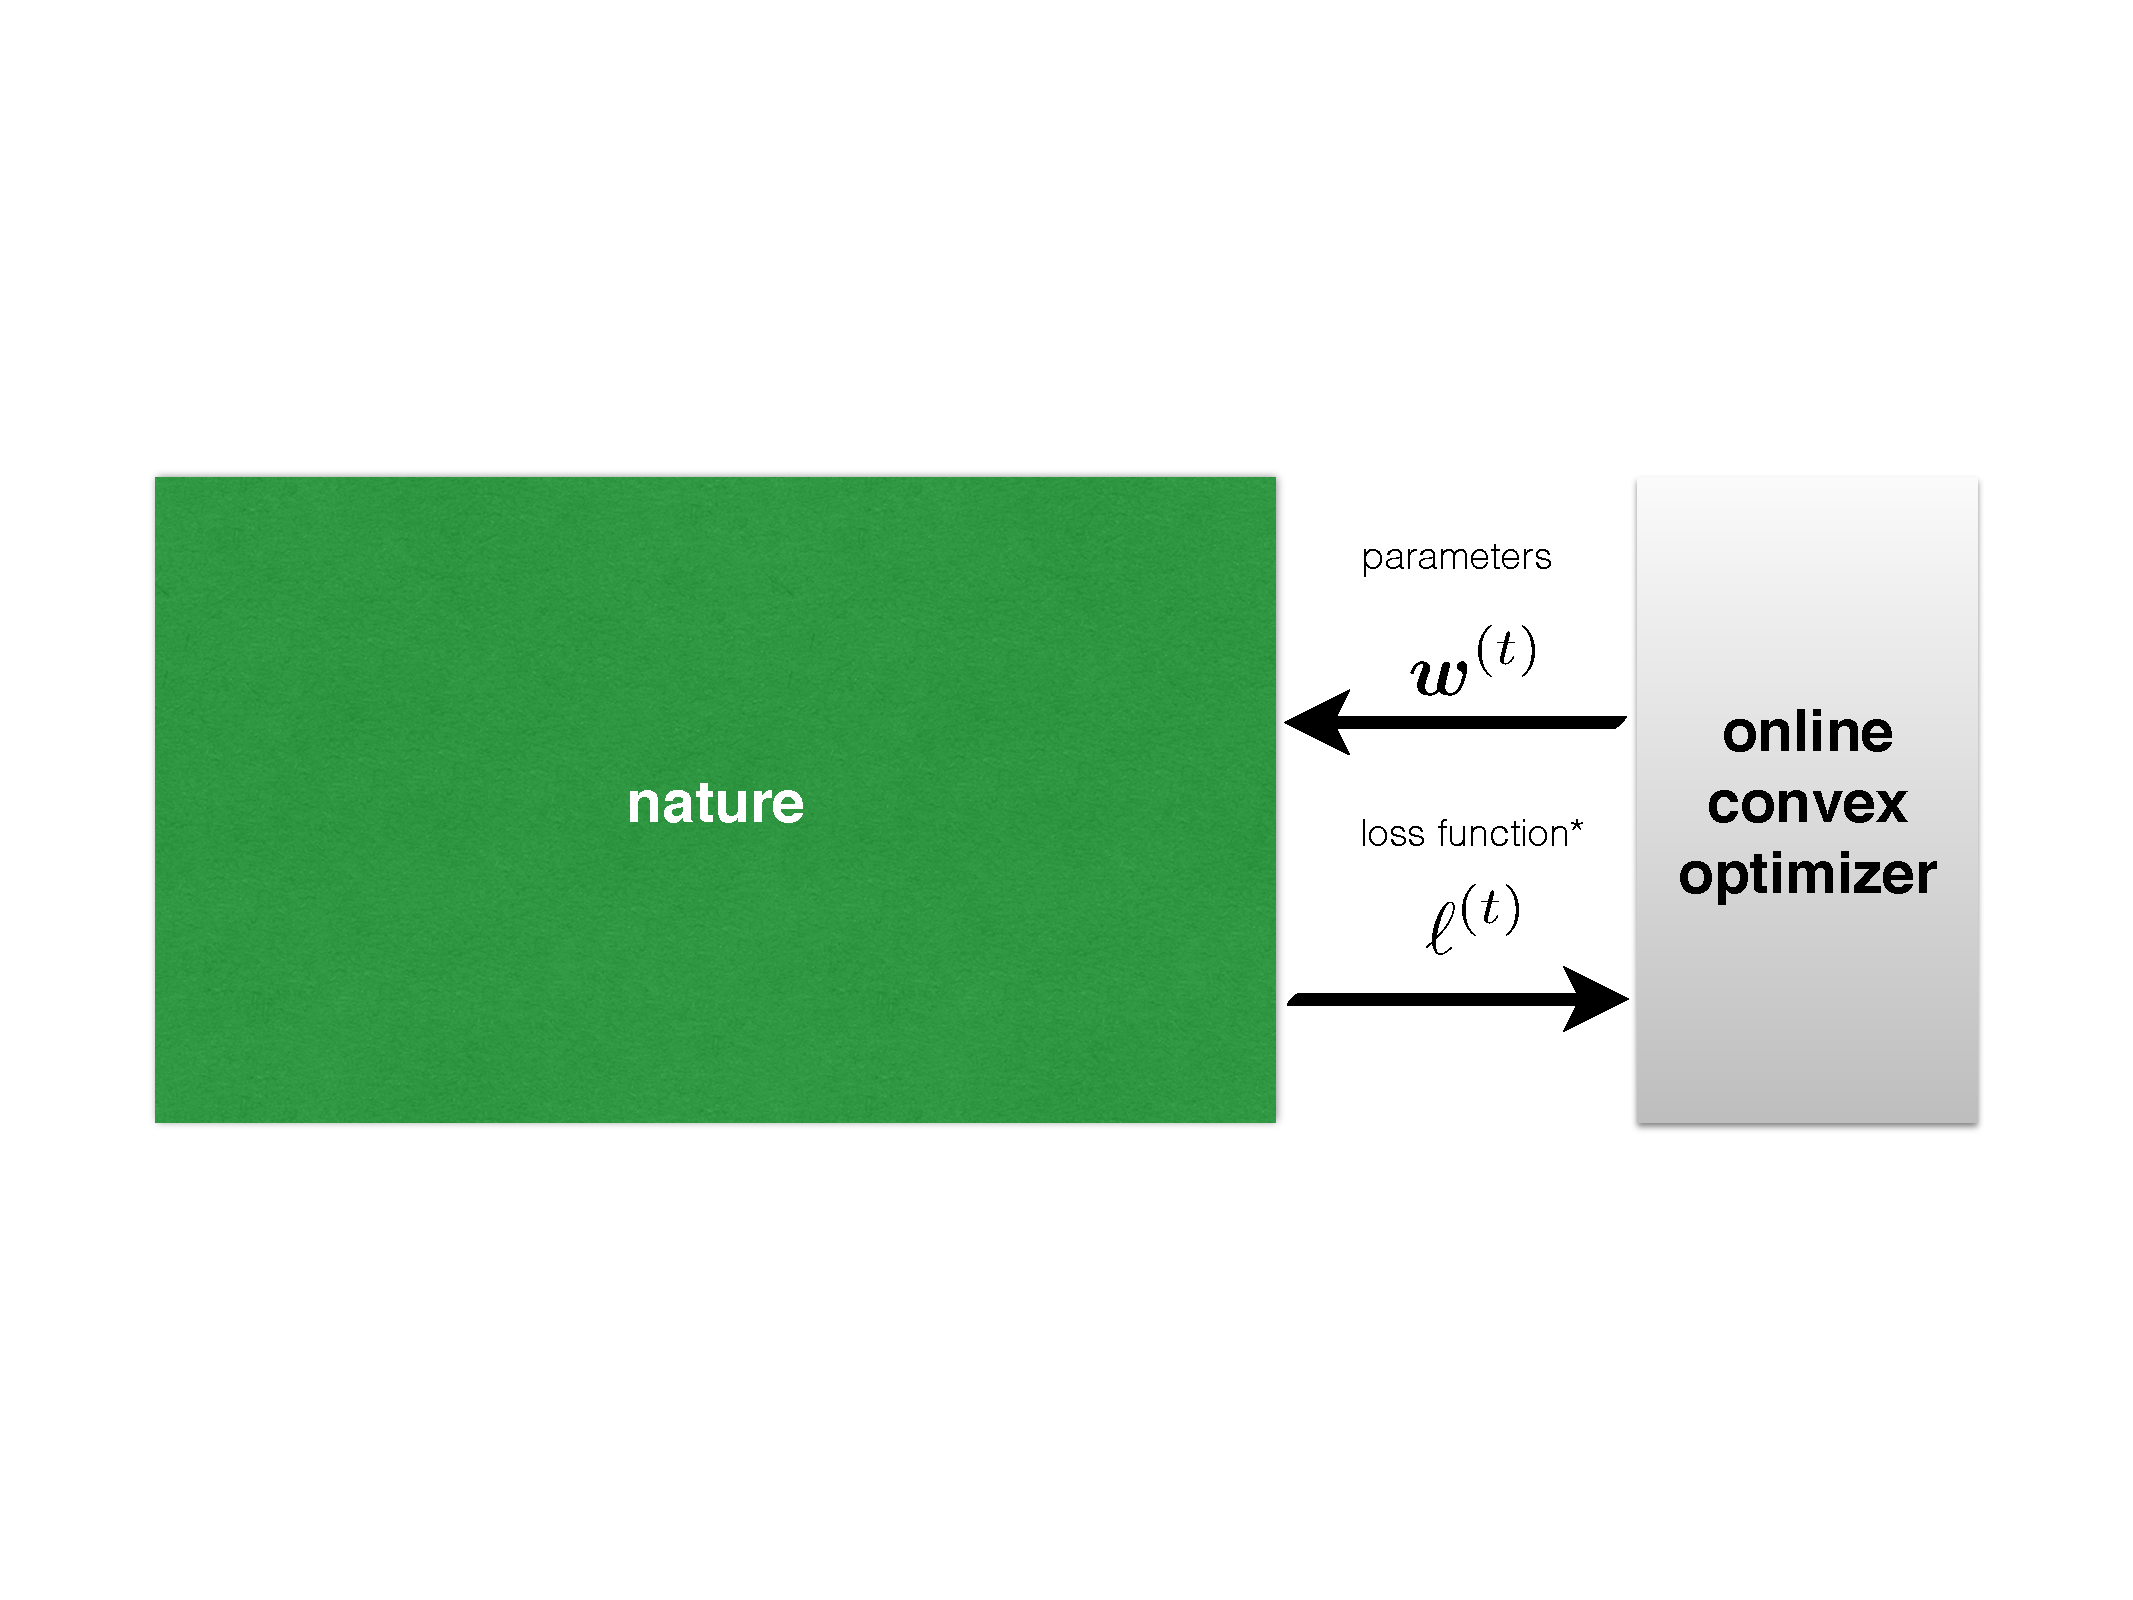
\includegraphics[width=\linewidth]{figure/oco_1.pdf}
    \caption{OCO framework}
    \label{fig:oco_1}
\end{minipage}%
\end{figure}

We introduced our first algorithm called \textit{Follow the Leader} (FTL) known as `Fictitious Play' (Brown 1951 \cite{berger2007brown}). The prediction rule is that the learner is going to choose the parameter $\bm{w}$ such that it minimizes the cumulative loss up to now. This rule can be inserted into the online convex optimizer in Fig. \ref{fig:oco_1}.\\
\begin{algorithm}
  \caption{FTL}\label{euclid}
  \begin{algorithmic}[1]
    \Function{Follow The Leader}{} %\Comment{The g.c.d. of a and b}
        \For{$t=1, 2,\,\cdots,\;T$}
            \State $\bm{w}^{(t)}$ = $\argmin{\bm{w} \in W} \Sigma^{t-1}_{i=1} f^{(i)} (\bm{w})$ \Comment{Parameter chosen}
            \State \textsc{Receive} ($f^{(t)} : W \rightarrow \mathbb{R}$) \Comment{Receive loss function}
        \EndFor
    \EndFunction
  \end{algorithmic}
\end{algorithm}

We used ``the one-step look ahead cheater'' to upper bound the regret:   

\begin{equation*}
    R(\bm{u}) = \sum_{t}[f^{(t)}(\bm{w}^{(t)}) - f^{(t)}(\bm{u})] \leq \sum_{t}[f^{(t)}(\bm{w}^{(t)}) - f^{(t)}(\bm{w}^{(t+1)})]
\end{equation*}

In this lecture, we study the FTL algorithm with different loss functions. We will see how linear loss function will make the FTL unstable and then introduce regularization to resolve such instability.

\section{Types of Loss Functions}
In the ``Follow the leader'' algorithm, the environment returns a loss function. Loss functions affect the algorithm's performance guarantees. Fig. \ref{fig:zero_one_loss} shows some examples of loss functions.
\begin{figure}[h]
    \centering
    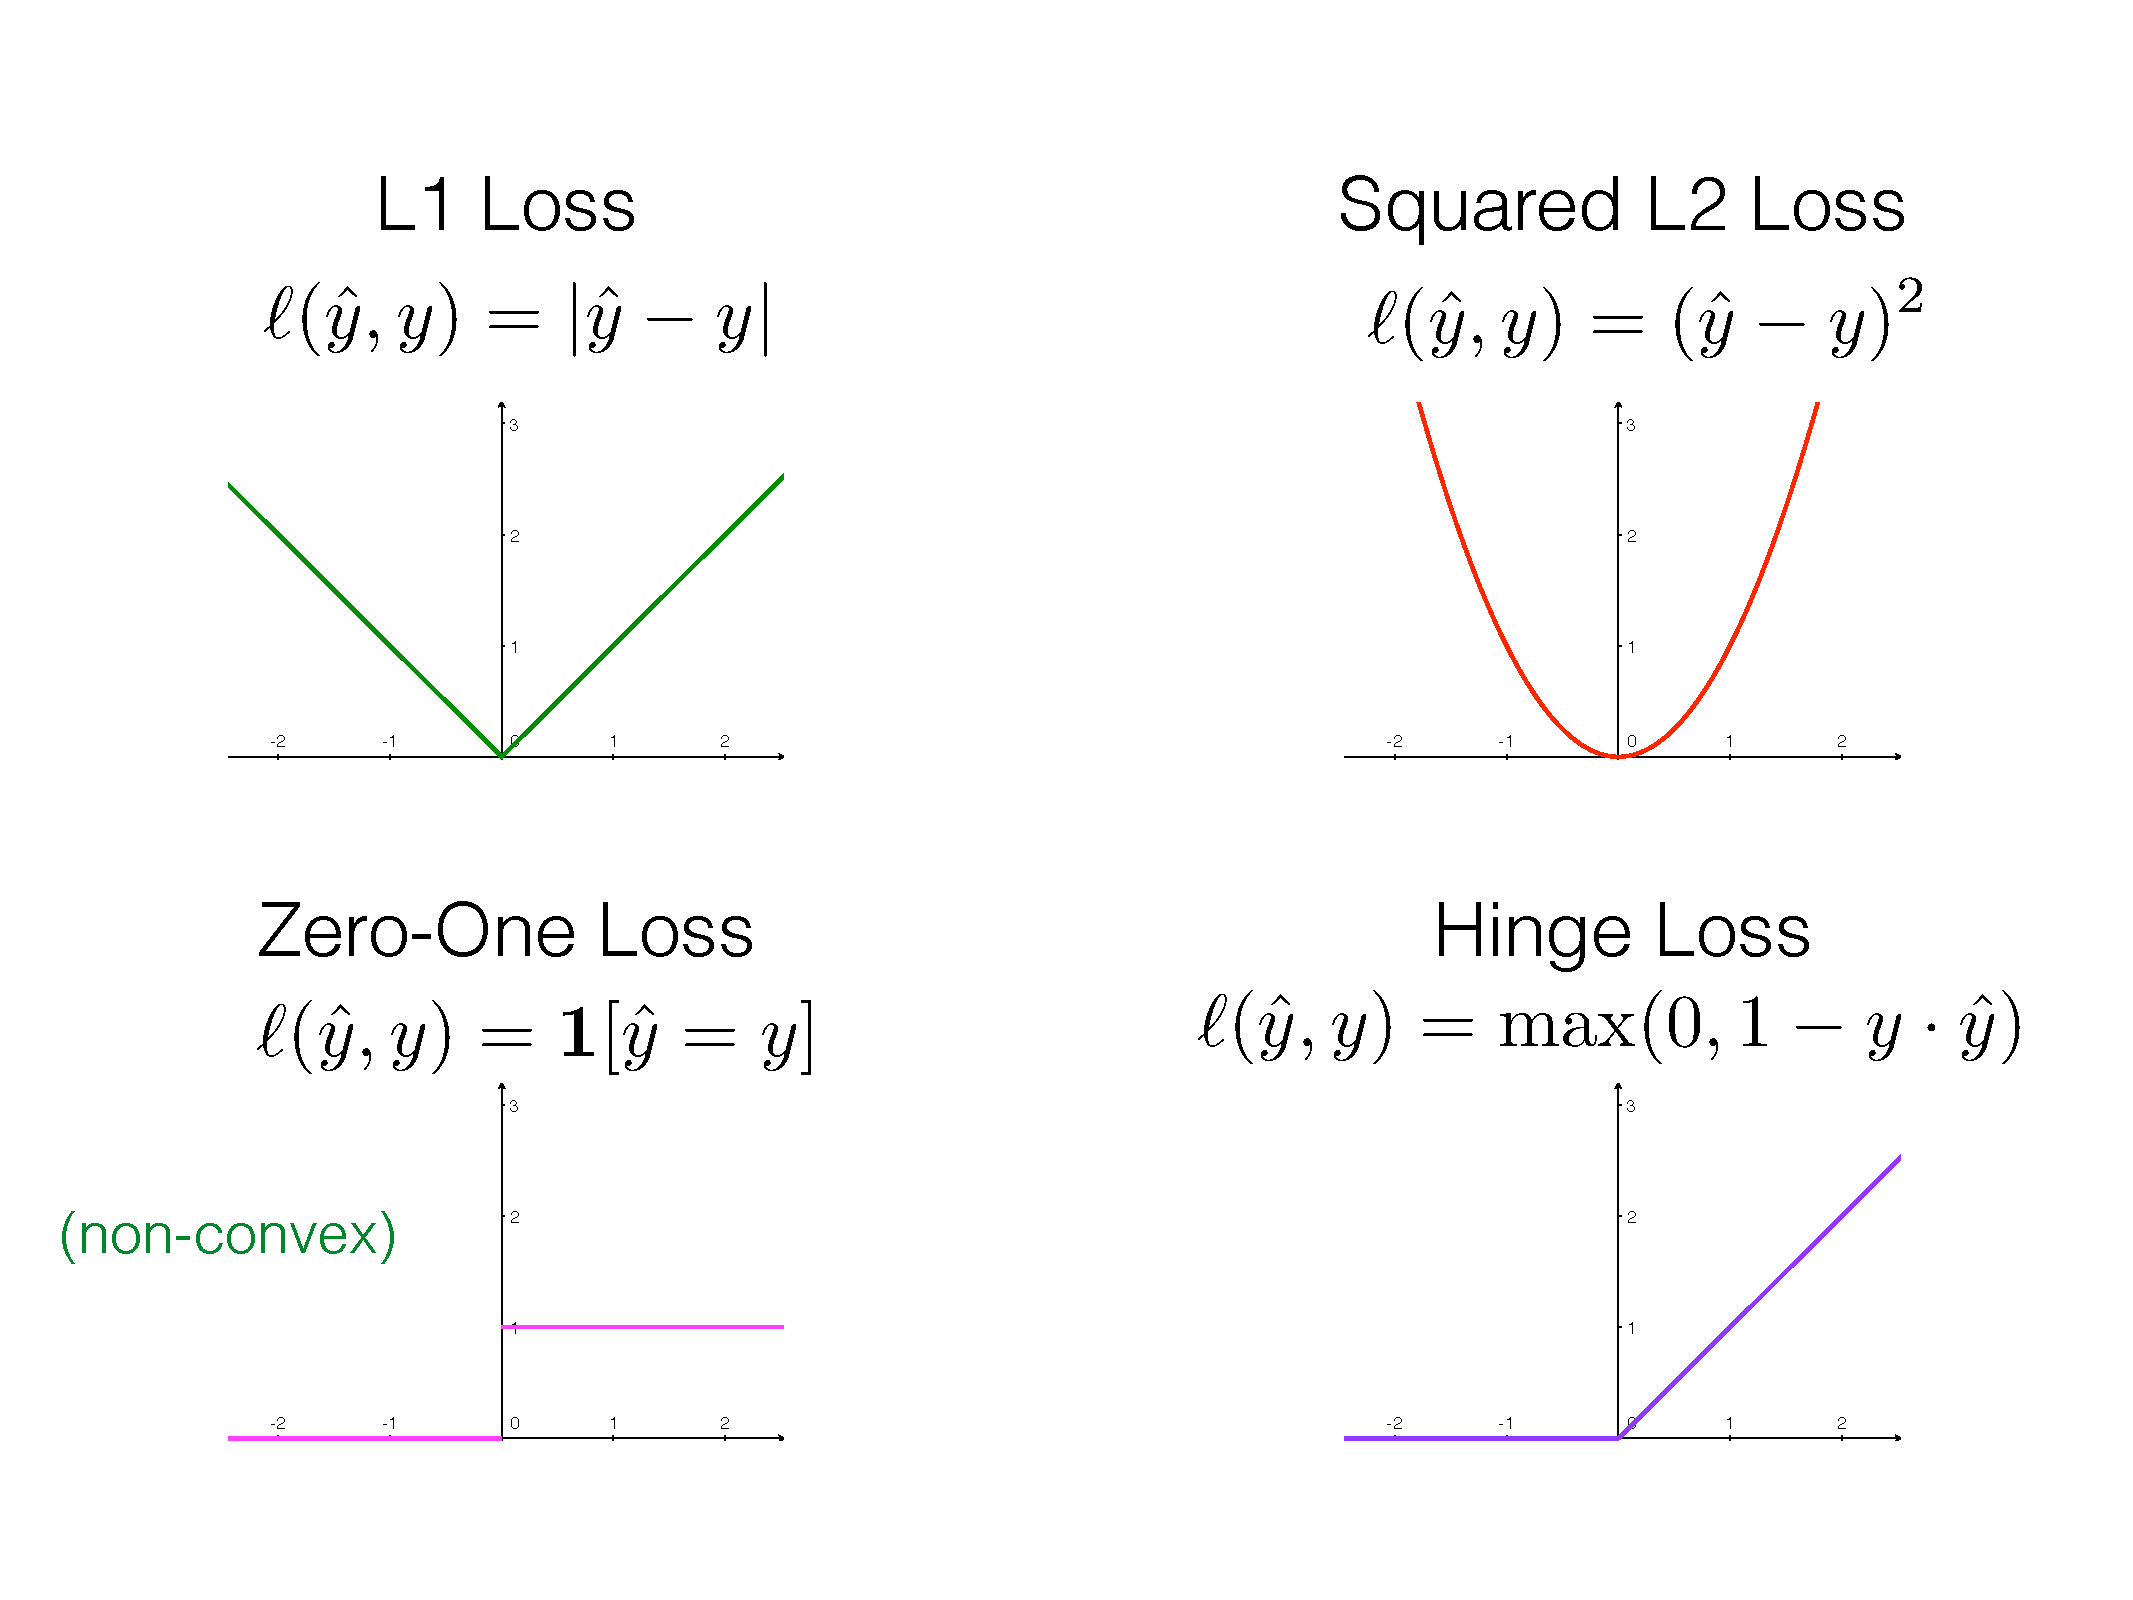
\includegraphics[width=0.8\textwidth]{figure/loss_func.pdf}
    \caption{Many types of loss function}
    \label{fig:zero_one_loss}
\end{figure}\\

\noindent
In section \ref{sec:ftl_quad_loss}, we take a look at FTL with a quadratic (squared L2) loss function as a concrete example.

\section{Follow The Leader with Quadratic Loss}
\label{sec:ftl_quad_loss}

\begin{algorithm}
  \caption{FTL with Quadratic Loss}\label{euclid}
  \begin{algorithmic}[1]
    \Function{Follow the leader (Quadratic Loss)}{} %\Comment{The g.c.d. of a and b}
    \State $f^{(0)} \leftarrow 0$
        \For{$t=1, 2,\,\cdots,\;T$}
            \State $\bm{w}^{(t)}$ = $\argmin{\bm{w} \in S} \Sigma^{t-1}_{i=1} f^{(i)} (\bm{w})$ 
            \State \textsc{Receive} ($f^{(t)} = \frac{1}{2}||\bm{w} - \bm{z}^{(t)}||_2^2$) \Comment{Receive loss function}
        \EndFor
    \EndFunction
  \end{algorithmic}
\end{algorithm}
 
\noindent In this algorithm, the entire loss function comes from the environment. $\bm{z}$ is a parameter of the loss function and $\bm{w}$ is the input. Since the average of $\bm{z}$ we have seen up to now is the minimizer of the quadratic loss, we can rewrite step 4 as:
\begin{equation*}
    \bm{w}^{(t)} = \frac{1}{t-1}\sum^{t-1}_{i=1}z^{(i)}
\end{equation*}

\subsection{Regret Bound}  
Assume that nature always chooses a quadratic loss:\\
\begin{equation*}
    f^{(t)}(w) = \frac{1}{2}||w - z^{(t)}||_2^2
\end{equation*}
We assume that points are bounded:\\
\begin{equation*}
    ||z||^2_2 \leq L
\end{equation*}
Recall that our generic FTL regret bound is:\\
\begin{equation*}
    R(\bm{u}) = \sum_{t}[f^{(t)}(\bm{w}^{(t)}) - f^{(t)}(\bm{u})] \leq \sum_{t}[f^{(t)}(\bm{w}^{(t)}) - f^{(t)}(\bm{w}^{(t+1)})]
\end{equation*}
Now we inset the quadratic loss into the right hand side of the bound:\\
\begin{equation*}
\begin{aligned}
     f^{(t)}(w^{(t)}) - f^{(t)}(w^{(t+1)}) = \frac{1}{2}||w^{(t)} - z^{(t)}||_2^2 - \frac{1}{2}||w^{(t+1)} - z^{(t)}||_2^2 \\ = \frac{1}{2}||w^{(t)} - z^{(t)}||_2^2 - \frac{1}{2}||(1-\frac{1}{t})w^{(t)} + (\frac{1}{t})z^{(t)} - z^{(t)}||_2^2
\end{aligned}
\end{equation*}
Recall that mean of $z$ is the quadratic loss minimizer:\\
\begin{equation*}
    w^{(t)} = \frac{1}{t-1}\sum^{t-1}_{i=1}z^{(i)}
\end{equation*}
We can convert it in a incremental, then we have the update step:\\
\begin{equation*}
    w^{(t+1)} = (1-\frac{1}{t})w^{(t)} + (\frac{1}{t})z^{(t)}
\end{equation*}
Now we plug in minimizer and upper-bound it:\\
\begin{equation*}
\begin{aligned}
     f^{(t)}(w^{(t)}) - f^{(t)}(w^{(t+1)}) &= \frac{1}{2}||w^{(t)} - z^{(t)}||_2^2 - \frac{1}{2}||(1-\frac{1}{t})w^{(t)} + (\frac{1}{t})z^{(t)} - z^{(t)}||_2^2 \\ 
     &= \frac{1}{2}\left(1 - (1 - \frac{1}{t})^2\right)||w^{(t)} - z^{(t)}||_2^2
\end{aligned}
\end{equation*}

Use the `known' inequality:\\
\begin{equation*}
    \frac{1}{2}\left(1 - (1 - \frac{1}{t})^2\right) \leq \frac{1}{t}
\end{equation*}

We can have:\\
\begin{equation*}
\begin{aligned}
     f^{(t)}(w^{(t)}) - f^{(t)}(w^{(t+1)}) \leq \left(\frac{1}{t}\right)||w^{(t)} - z^{(t)}||_2^2
\end{aligned}
\end{equation*}

Recall our prior assumptions:\\
\begin{equation*}
    L = \max \limits_{t}||z^{(t)}||
\end{equation*}
Since average is less or equal to max, we have:\\
\begin{equation*}
    ||w^{(t)}|| \leq L
\end{equation*}
Based on triangle inequality, we can get:\\
\begin{equation*}
    ||w^{(t)} - z^{(t)}|| \leq 2L
\end{equation*}
Therefore, we have:\\
\begin{equation*}
    f^{(t)}(w^{(t)}) - f^{(t)}(w^{(t+1)}) \leq \left(\frac{1}{t}\right) 4L^2
\end{equation*}
Recall the regret bound over all time steps is:\\
\begin{equation*}
    R(\bm{u}) \leq \sum_{t}[f^{(t)}(\bm{w}^{(t)}) - f^{(t)}(\bm{w}^{(t+1)})] 
\end{equation*}
We know another useful approximation:\\
\begin{equation*}
    \sum_{t=1}^T \leq 1 + \int_1^T (1/t) dt = \log(T) + 1 
\end{equation*}
Therefore, the regret bound is:\\
\begin{equation*}
    \text{Regret} \leq 4L^2 \left( \log(T) + 1 \right)
\end{equation*}

This is no-regret since the average regret grows sub-linearly in T. However, this only holds for quadratic loss functions, not for all convex functions.\\

\section{Follow The Leader with Linear Loss}
\label{sec:ftl_linear_loss}

\begin{algorithm}
  \caption{Follow the leader algorithm with linear loss}\label{euclid}
  \begin{algorithmic}[1]
    \Function{Follow the leader (Linear Loss)}{} %\Comment{The g.c.d. of a and b}
        \For{$t=1, 2,\,\cdots,\;T$}
            \State $\bm{w}^{(t)}$ = $\argmin{\bm{w} \in S} \left(\Sigma^{t-1}_{i=1} \bm{z}^{(i)}\right) \cdot \bm{w}$ 
            \State \textsc{Receive} ($f^{(t)}(\bm{w}) = \bm{z}^{(t)} \cdot \bm{w}$) \Comment{Receive loss function}
        \EndFor
    \EndFunction
  \end{algorithmic}
\end{algorithm}
In this algorithm, the space of possible predictions is $\bm{w} \in S = [-1, 1]$. The nature always chooses a linear loss: $f^{(t)}(\bm{w}) = \bm{z}^{(t)} \cdot \bm{w}$, where $\bm{z}^{(t)} =\left\{
\begin{array}{rcl}
-0.5       &      & \text{if t is 1}\\
1     &      & \text{if t is even}\\
-1     &      & \text{if t is odd}\\
\end{array} \right. $\\
The total loss of this FTL learner is:\\
\begin{equation*}
    L = \sum_{t=1}^T f^{(t)} = \sum_{t=2}^T 1 = T -1
\end{equation*}
The total loss of expert $u=0$:\\
\begin{equation*}
    L_u = \sum_{t=2}^T z^{(t)} \cdot u = \sum_{t=2}^T 0= 0
\end{equation*}
The regret of FTL with linear loss relative to expert $u$ that chooses $w=0$:\\
\begin{equation*}
    \text{Regret}(u) = T-1-0 = T-1 = O(T)
\end{equation*}
The regret grows linearly. It is because the $\bm{w}$ value flip-flops back and forth to make the algorithm unstable. To resolve this issue, we will introduce regularization in next section. 


\section{Follow The Regularized Leader}

In section \ref{sec:ftl_linear_loss} we saw that FTL with linear loss is very unstable. To make $\bm{w}$ more stable, here we introduce the \textit{Follow the Regularized Leader} (FTRL) algorithm.

\begin{algorithm}
  \caption{Follow The Regularized Leader}\label{euclid}
  \begin{algorithmic}[1]
    \Function{FTRL(Convex Set $\mathcal{S}$)}{} %\Comment{The g.c.d. of a and b}
    \For{$t=1, 2,\,\cdots,\;T$}
        \State $\bm{w}^{(t)}$ = $\argmin{\bm{w} \in S} \Sigma^{t-1}_{i=1} f^{(i)} (\bm{w}) + \psi(\bm{w})$
        \Comment{Added $\psi(\bm{w})$ to the prediction rule}
        \State \textsc{Receive} ($f^{(t)} : \mathcal{S} \rightarrow \mathbb{R}$)
    \EndFor
    \EndFunction
  \end{algorithmic}
\end{algorithm}

Note that FTL is just FTRL with $\psi = 0$.

\subsection{Regret Bound}
The regret bound for FTRL is similar to that of the FTL, with an additional term due to regularization:
\begin{align*}
    R(\bm{u}) &\triangleq \sum_{t=1}^{T} \left[ f^{(t)}(\bm{w}^{(t)}) - f^{(t)}(\bm{u}) \right]\\
    & \leq \left[ \psi(\bm{u}) - \psi(\bm{w}^{(1)}) \right] +  \sum_{t=1}^{T} \left[ f^{(t)}(\bm{w}^{(t)}) - f^{(t)}(\bm{w}^{(t+1)}) \right]
\end{align*}
\begin{proof}
Given the regret bound for FTL using one-step look ahead cheater:
\begin{align}
    \notag
    R(\bm{u}) &= \sum_{t=1}^T \left[ f^{(t)}(\bm{w}^{(t)}) - f^{(t)}(\bm{u}) \right]\\
    &\leq \sum_{t=1}^T \left[ f^{(t)}(\bm{w}^{(t)}) - f^{(t)}(\bm{w}^{(t+1)}) \right]
    \label{eqn:ftl_regret_bound}
    \intertext{Add the $t=0$ 'loss' for FTRL on both sides of (\ref{eqn:ftl_regret_bound}):}
    \notag
    \left[ f^{(0)}(\bm{w}^{(0)}) - f^{(0)}(\bm{u})\right] &+
    \sum_{t=1}^T \left[ f^{(t)}(\bm{w}^{(t)}) - f^{(t)}(\bm{u}) \right]\\
    &\leq \left[ f^{(0)}(\bm{w}^{(0)}) - f^{(0)}(\bm{u})\right] +
    \sum_{t=1}^T \left[ f^{(t)}(\bm{w}^{(t)}) - f^{(t)}(\bm{w}^{(t+1)}) \right]
    \intertext{Swap in the regularizer notation:}
    \notag
    \left[ \phi(\bm{w}^{(0)}) - \phi(\bm{u})\right] &+
    \sum_{t=1}^T \left[ f^{(t)}(\bm{w}^{(t)}) - f^{(t)}(\bm{u}) \right]\\
    &\leq \left[ \phi(\bm{w}^{(0)}) - \phi(\bm{u})\right] +
    \sum_{t=1}^T \left[ f^{(t)}(\bm{w}^{(t)}) - f^{(t)}(\bm{w}^{(t+1)}) \right]
    \intertext{Subtract $\phi(\bm{w}^{(0)}) - \phi(\bm{u})$ from both sides:}
    \sum_{t=1}^{T} \left[ f^{(t)}(\bm{w}^{(t)}) - f^{(t)}(\bm{u}) \right]
    & \leq \left[ \psi(\bm{u}) - \psi(\bm{w}^{(1)}) \right] +  \sum_{t=1}^{T} \left[ f^{(t)}(\bm{w}^{(t)}) - f^{(t)}(\bm{w}^{(t+1)}) \right]
\end{align}
\end{proof}

\subsection{FTRL with Linear Loss}
Now we revisit the linear loss function scenario and see if FTRL can make $\bm{w}$ more stable using quadratic regulation. We use a squared L2 norm as a quadratic regularizer:
\begin{equation}
    \phi(\bm{w}) = \frac{1}{2\eta} ||\bm{w}||^2_2
\end{equation}
The linear loss function is the same as before:
\begin{equation}
    f^{(t)} = \bm{w} \cdot z^{(t)}
\end{equation}

\begin{algorithm}[h]
  \caption{FTRL with Linear Loss And Quadratic Regulation}\label{euclid}
  \begin{algorithmic}[1]
    \Function{FTRL(Convex Set $\mathcal{S}$)}{} %\Comment{The g.c.d. of a and b}
    \For{$t=1, 2,\,\cdots,\;T$}
        \State $\bm{w}^{(t)}$ = $\argmin{\bm{w} \in S} \Sigma^{t-1}_{i=1} \left( \frac{1}{2\eta} ||\bm{w}||^2_2 + \bm{w} \cdot \sum_{i=1}^{t-1} z^{(i)} \right)$
        \Comment{Prediction rule}
        \State \textsc{Receive} ($f^{(t)} : \bm{w} \cdot z^{(t)}$)
    \EndFor
    \EndFunction
  \end{algorithmic}
\end{algorithm}
With quadratic regularization, the prediction rule now becomes an unconstrained quadratic programming problem. For convenience of analysis, we introduce the following short-hand for the sum:
\begin{equation}
    \theta^{(t)} = \sum_{i=1}^{t-1} z^{(i)}
    \label{eqn:short_hand}
\end{equation}
We will later see that $\theta^{(t)}$ is the sum of loss function gradients. With this short-hand, we can write the prediction rule as:
\begin{equation}
    \bm{w}^{(t)} = \argmin{\bm{w} \in S} \Sigma^{t-1}_{i=1} \left( \frac{1}{2\eta} ||\bm{w}||^2_2 + \bm{w} \cdot \theta^{(t)} \right)
    \label{eqn:ftrl_lq_pred_rule}
\end{equation}
To minimize the quadratic function in (\ref{eqn:ftrl_lq_pred_rule}), we calculate its first derivative and set to zero:
\begin{align}
    \notag
    \frac{d}{d\bm{w}} \left( \frac{1}{2\eta}||\bm{w}||^2_2 + \bm{w} \cdot \theta^{(t)} \right) &= 0\\
    \notag
    \frac{1}{2\eta} 2 \bm{w} + \theta^{(t)} &= 0\\
    \notag
    \bm{w} &= -\eta \theta^{(t)}\\
    \intertext{Substitute (\ref{eqn:short_hand}):}
    \notag
    \bm{w}^{(t)} &= -\eta \sum_{i=1}^{t-1} z^{(i)}\\
    \notag
    &= -\eta \left( \sum_{i=1}^{t-2} z^{(i)} + z^{(t-1)} \right)\\
    \notag
    &= -\eta \sum_{i=1}^{t-2} z^{(i)} - \eta z^{(t-1)}\\
    \label{eqn:ftrl_quad_update}
    &= \bm{w}^{(t-1)} - \eta z^{(t-1)}
\end{align}
Note that (\ref{eqn:ftrl_quad_update}) is an update equation for $\bm{w}$ across each iteration. The hyper parameter $\eta$ controls the step size / learning rate. This convenience of doing optimization with incremental updates is really due to the fact that we chose a good regularizer function. Otherwise we would have had to solve a full optimization problem in each iteration.

Also note that we have seen a similar form of (\ref{eqn:ftrl_quad_update}) before in the perceptron algorithm. We will see this update form again in future gradient descent algorithms and the general form of this update equation is called online gradient descent:
\begin{equation}
    \label{eqn:ftrl_update_general}
    \bm{w}^{(t)} = \bm{w}^{(t-1)} - \eta \nabla f^{(t-1)}
\end{equation}

\subsection{Regret of FTRL with Euclidean Regularizer and Linear Loss}

The regret bound for FTRL with a Euclidean regularizer and linear loss function is:
\begin{equation}
    \label{eqn:ftrl_regret_bound_euclidean}
    R^{(T)}(\bm{u}) \leq BL\sqrt{2T}
\end{equation}
Where $L = \max_\mathcal{Z} || \mathcal{Z} ||_2$ and $B = \max_{\bm{u} \in \mathcal{S}} || \bm{u} ||_2$

\begin{proof}
\begin{align}
    \notag
    R^{(T)}(\bm{u}) &\leq \left[ \phi(\bm{u}) - \phi(\bm{w}^{(1)}) \right] +
    \sum_{t=1}^T \left[  f^{(t)} (\bm{w}^{(t)}) - f^{(t)}(\bm{w}^{(t+1)}) \right]
    & \text{Generic form}\\
    \notag
    &= \left[  \frac{1}{2\eta}||\bm{u}||^2_2 - 0 \right] +
    \sum_{t=1}^T \left[ \langle \bm{w}^{(t)}, \bm{z}^{(t)} \rangle - \langle \bm{w}^{(t+1)}, \bm{z}^{(t)}\rangle \right]
    & \text{Plug in regularizer}\\
    \notag
    &= \frac{1}{2\eta}||\bm{u}||^2_2 + \sum_{t=1}^T \langle \bm{w}^{(t)} - \bm{w}^{(t+1)}, \bm{z}^{(t)} \rangle
    & \text{Rearrangement} \\
    \notag
    &= \frac{1}{2\eta}||\bm{u}||^2_2 + \sum_{t=1}^T \eta || \bm{z}^{(t)} ||^2\\
    \intertext{So we have the following regret bound:}
    \notag
    R^{(T)}(\bm{u}) &\leq \frac{1}{2\eta}||\bm{u}||^2_2 +
    \sum_{t=1}^T \eta || \bm{z}^{(t)} ||^2\\
    \notag
    R^{(T)}(\bm{u}) &\leq \frac{1}{2\eta}B^2 + \eta T L^2\\
    \notag
    R^{(T)}(\bm{u}) &\leq BL \sqrt{2T}
    & \text{Optimal value at $\eta = \frac{B}{L \sqrt{2T}}$}
\end{align}
\end{proof}

Because the regret bound (\ref{eqn:ftrl_regret_bound_euclidean}) is sub-linear, FTRL with an Euclidean regualizer and linear loss is a no regret algorithm.

Now that we have studied the FTRL framework, looking back at the online perceptron algorithm and RWMA, their update rules actually come from the general form of FTRL update rule (\ref{eqn:ftrl_update_general}). This is illustrated in Fig. \ref{fig:ftrl_examples} Specifically, both online perceptron algorithm and RWMA have linear loss. Their difference is that the online perceptron algorithm uses an Euclidean regularization but the RWMA uses an Entropic regularization.

\begin{figure}[h]
    \centering
    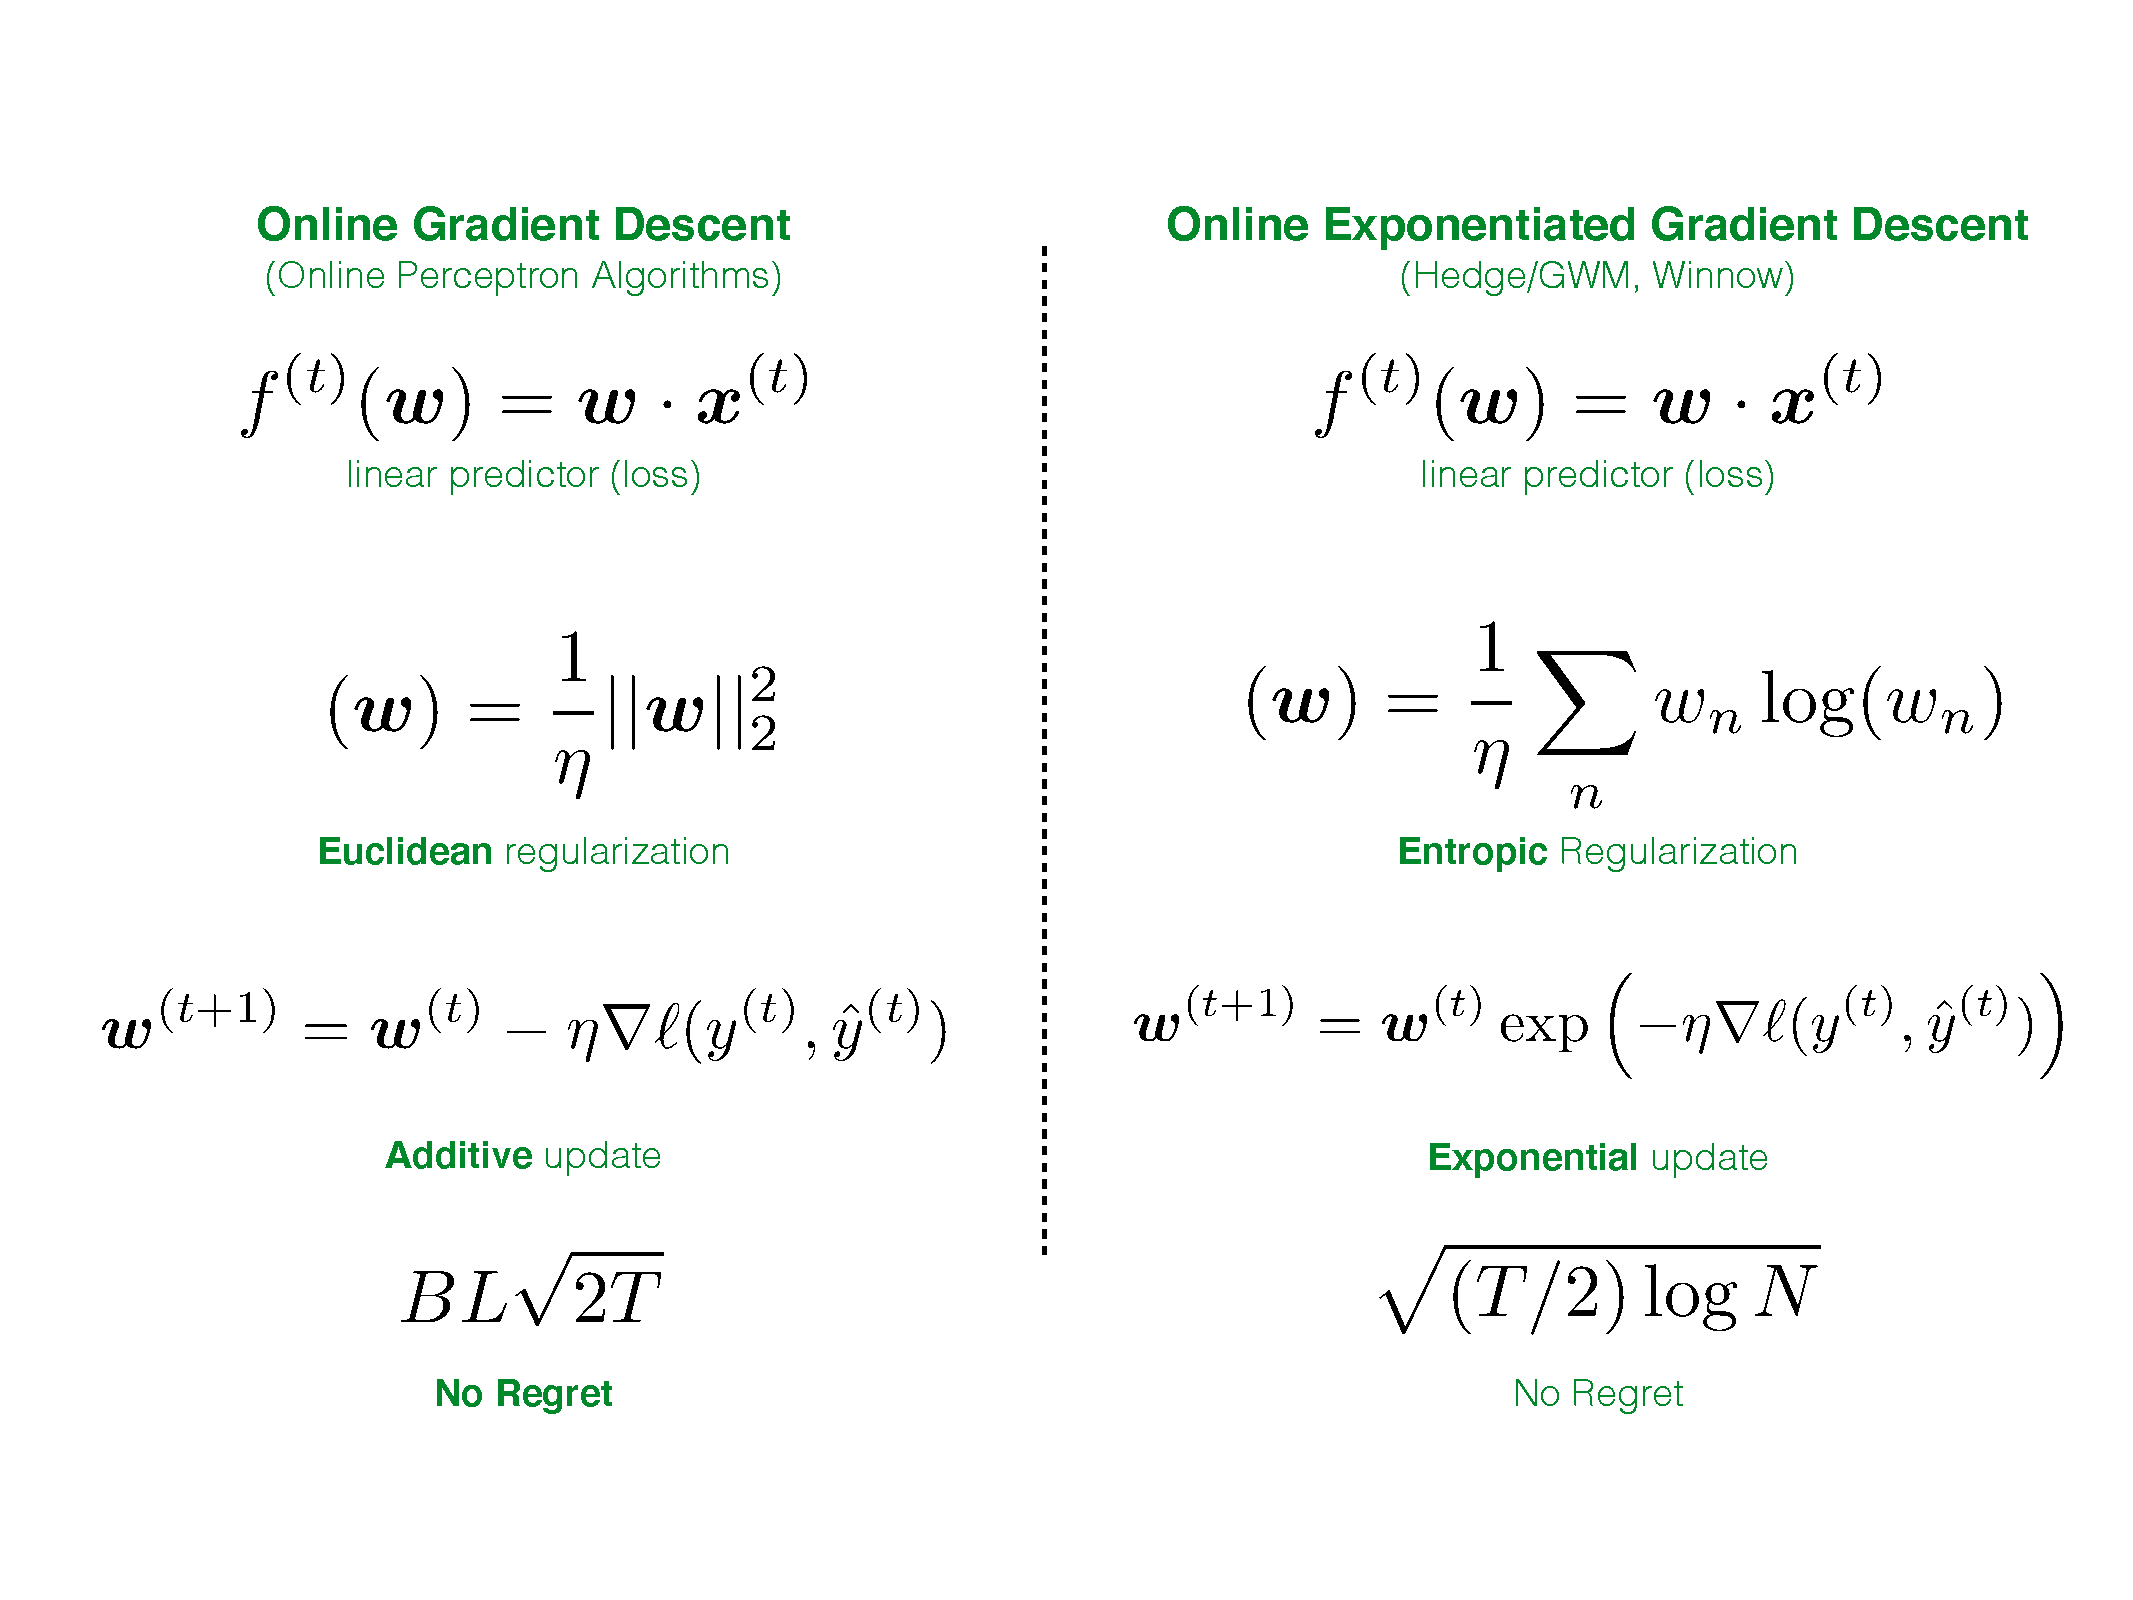
\includegraphics[width=\textwidth]{figure/ftrl_examples.pdf}
    \caption{FTRL examples that we have seen before}
    \label{fig:ftrl_examples}
\end{figure}

\section{Online Mirror Descent}
\textit{Online Mirror Descent} (OMD) can be considered as a special case of FTRL with a linear loss and a convex regularizer. Because we did not finish discussing OMD in the lecture, details on OMD will be covered in our next scribe notes.

\newpage

%\section*{References}
%Include your references here. Please cite any resources you found useful.	
%Populate the refs.bib file or list your references manually. Be consistent in formatting!
{
\bibliography{refs}
\bibliographystyle{abbrv}
}

%\section{Appendix}
%This section provides any relevant background material that was not covered in the lectures, but was found to be useful for understanding the material. 
%For example, derivations, theory underlying techniques employed, etc. 

%Additionally, this section can summarizes applications or extensions of these techniques found in the literature. 

\end{document} % Done!





